\documentclass[a4paper,11pt]{article}
\include{../../../latex_headers/lab_header}

% ---------------------------------- Document ----------------------------------
\begin{document}
\pagenumbering{arabic}

\begin{center}
{\Large CMPUT 350 Lab 3 Prep Problems}
\end{center}

% Add important dates, change TA, add TA tools

\linerule

In this problem we consider mathematical expressions that are recursively defined as follows:
\begin{itemize}
    \item Any C type int constant is an expression
    \item If E and F are expressions, then (E), (E+F), (E-F), (E*F), (E/F) are also expressions
    \item Nothing else is an expression
\end{itemize}

\textbf{Example}: 1, (((90))), (3+4), ((3-4)*(3+5)) are expressions, while (), )(, (1+ are not.

\medskip

As a member of a compiler team you are in charge of creating a data structure for storing such expressions. 
You decide to create a class for each type of expression listed in the recursive definition:

\[ \text{ConstExpr, ParenExpr, PlusExpr, MinusExpr, TimesExpr, DivExpr} \]

and deriving them from base-class Expr like so:

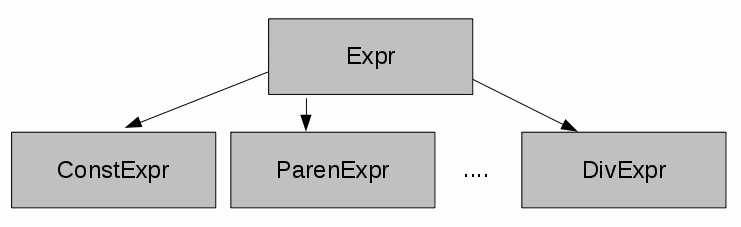
\includegraphics[width=0.8\linewidth]{tree.png}

Each sub-expression object either contains its value (ConstExpr) or pointers to one (ParenExpr) or two sub-expressions 
(PlusExpr,MinusExpr,TimesExpr,DivExpr).

\medskip

In addition to a value or pointers to sub-expressions, 
each expression object has a method called value() which recursively computes the value of the 
expression based on a stored value or 1 or 2 sub-expressions which are referred to by pointers 
stored in sub-expression objects. 
Each such pointer owns its pointee object, i.e., the expression destructors must call the pointee object destructors.


\begin{cppcode*}{fontsize=\scriptsize}
class Expr {
public:
  Expr() { }
  virtual ~Expr() { }
  // return value of expression
  virtual int value() const = 0;
  // we are underpaid and therefore refuse to implement the CC and AO
  Expr(const Expr &) = delete;
  Expr &operator=(const Expr &) = delete;
};
class ConstExpr : public Expr {
public:
    ConstExpr(int v) : val(v) { }
    int value() const override { return val; }
private:
    int val;
};
// ...
\end{cppcode*}

Here is sample code that invokes value() on a constant expression via a base class pointer (polymorphically):
\begin{cppcode*}{fontsize=\scriptsize,linenos=false}
Expr *A = new ConstExpr(9);
cout << A->value() << endl;     // prints 9
\end{cppcode*}

It will be useful to implement constructors that take pointers to sub-expressions as parameters and 
stores them in the class object like so:
\begin{cppcode*}{fontsize=\scriptsize,linenos=false}
PlusExpr(Expr *s1, Expr *s2) {
    succ1 = s1;
    succ2 = s2;
}
\end{cppcode*}

It also may be useful to define intermediate expression type BinaryExpr which implements common binary expression 
functionalities. E.g.

\begin{cppcode*}{fontsize=\scriptsize,linenos=false}
class PlusExpr : public BinaryExpr {
public:
  PlusExpr(Expr *s1, Expr *s2) : BinaryExpr(s1, s2) { }
    int value() const override {
        return succ1->value() + succ2->value();
    }
};
\end{cppcode*}

As an example, consider expression (10+(30*((5-3)))) that can be represented by 8 sub-expressions 
by reading the expression inside out:

\begin{verbatim}
    Expression                    value() result
    --------------------------------------------------------
    Expr *A = new ConstExpr(5);   // 5
    Expr *B = new ConstExpr(3);   // 3
    Expr *C = new MinusExpr(A,B); // A->value()-B->value() = 2
    Expr *D = new ParenExpr(C);   // C->value() = 2  
    Expr *E = new ConstExpr(30);  // 30
    Expr *F = new TimesExpr(E,D); // E->value()*D->value() = 60
    Expr *G = new ConstExpr(10);  // 10
    Expr *H = new PlusExpr(G,F);  // G->value()+F->value() = 70
\end{verbatim}

Calling \cppinline{H->value()} computes 70 by recursively calling \cppinline{value()} on all sub-expressions.
Calling \texttt{delete H} needs to recursively delete all allocated objects.

\medskip 

Your task is to implement the whole expression type hierarchy, including constructors, destructors, and the \cppinline{value()} function.
AOs and CCs don't have to be implemented, but make sure that they can't be invoked by accident.
Also, use \texttt{valgrind} to ensure your implementation doesn't leak memory.


\end{document}